\documentclass[a4paper]{report}

% load packages
%\usepackage{showframe}
\usepackage[utf8]{inputenc}
\usepackage{enumitem}
\usepackage{listings}
\usepackage{courier}
\usepackage{hyperref}
\usepackage{graphicx}
\usepackage{float}
\usepackage[export]{adjustbox}

\setlength{\parskip}{1em}

\lstset{
  breaklines=true,
  basicstyle=\ttfamily,
  showstringspaces=false
}

\begin{document}

\title{Report of Programming Assignment 3 for CS 6301.001: Special Topics in Computer Science --- Introduction to Multi-Core Programming}

\author{Siming Liu}

\maketitle{}

\section*{Experiment Objective}
The experiment is intended to compare performance of two different implementations of concurrent unbounded queue. There are locked and lock-free version.

\section*{Experimental Environment}
Experiments run on a visualization node of \href{https://www.tacc.utexas.edu/}{TACC} distributed supercomputer clusters.
A visualization node have 2 Intel Xeon E5-2680 processors (x86\_64 architecture, 16 total cores) and 32GB of memory.
The operating system of a node runs is CentOS 6.8 with Linux kernel version 2.6.32.
Programming language of implementation is \lstinline{C++}.
The performance is compared with respect to system throughput with two parameters:
\begin{enumerate}
  \item distribution of various operations:
  \begin{itemize}
    \item write-dominated: 50\% enque, 50\% deque and 0\% is-empty
    \item mixed: 40\% enque, 40\% deque and 20\% is-empty
  \end{itemize}
  \item degree of concurrency: it varies the number of threads from one to twice the number of cores in a node. (aka $1 \sim 32$)
\end{enumerate}

\section*{Experimental Method}
In order to limit the maximum size of queue to 1000 keys, we set the maximum operations number to 2000.
For each type of throughput, we randomly generate 2000 operations according to the profile and then distribute these operations randomly to each thread as parameter. For each implementation, we launch $1 \sim 32$ threads to execution all 2000 operations and we do this 16 times to get average running time of all threads in nanosecond. So command \lstinline{concurrent_unbounded_queue 32 2000 16 9} are used to launch testing, in which 32 is maximum thread number, 2000 is operation number, 16 is repeated times and 9 is maximum key value.

\section*{How to Test Correctness}
For each operation of each thread, we log on the invocation and response event. The macro \lstinline{CALL_FUNC_IF_MATCH} is intended for this logging. So for each unit test, we can get a concurrent history of all threads. And we manually check all concurrent histories to see whether they are all linearizability. If all the concurrent histories tested of a implementation are linearizability, we can say the implementation is correct with high probability. In order to achieve that and conveniently for manually checking, we use command \lstinline{concurrent_unbounded_queue 5 20 1 100} to test correctness. Below is a part of actual test result to just show the idea. Whole correctness verfication needs thorough tests. It is a concurrent history of lock-free version with $5$ threads and $20$ operations. We can see it is linearizability.

\begin{lstlisting}[basicstyle=\ttfamily\scriptsize]
--- [LockFreeQueue] Thread = 5 Concurrent History ---
[thread 0] LockFreeQueue::Deque()
[thread 0] LockFreeQueue::Deque() = empty
[thread 1] LockFreeQueue::Enque(59)
[thread 1] LockFreeQueue::Enque(59) = void
[thread 1] LockFreeQueue::Deque()
[thread 1] LockFreeQueue::Deque() = 59
[thread 1] LockFreeQueue::Deque()
[thread 3] LockFreeQueue::Deque()
[thread 1] LockFreeQueue::Deque() = empty
[thread 1] LockFreeQueue::IsEmpty()
[thread 1] LockFreeQueue::IsEmpty() = true
[thread 4] LockFreeQueue::Deque()
[thread 3] LockFreeQueue::Deque() = empty
[thread 0] LockFreeQueue::Enque(83)
[thread 4] LockFreeQueue::Deque() = empty
[thread 2] LockFreeQueue::Enque(81)
[thread 4] LockFreeQueue::Deque()
[thread 4] LockFreeQueue::Deque() = 83
[thread 2] LockFreeQueue::Enque(81) = void
[thread 2] LockFreeQueue::Enque(31)
[thread 2] LockFreeQueue::Enque(31) = void
[thread 2] LockFreeQueue::Enque(72)
[thread 2] LockFreeQueue::Enque(72) = void
[thread 2] LockFreeQueue::Deque()
[thread 2] LockFreeQueue::Deque() = 81
[thread 3] LockFreeQueue::Deque()
[thread 4] LockFreeQueue::IsEmpty()
[thread 0] LockFreeQueue::Enque(83) = void
[thread 0] LockFreeQueue::Enque(4)
[thread 0] LockFreeQueue::Enque(4) = void
[thread 0] LockFreeQueue::Enque(60)
[thread 0] LockFreeQueue::Enque(60) = void
[thread 3] LockFreeQueue::Deque() = 31
[thread 4] LockFreeQueue::IsEmpty() = false
[thread 3] LockFreeQueue::Enque(71)
[thread 4] LockFreeQueue::IsEmpty()
[thread 3] LockFreeQueue::Enque(71) = void
[thread 4] LockFreeQueue::IsEmpty() = false
[thread 3] LockFreeQueue::IsEmpty()
[thread 3] LockFreeQueue::IsEmpty() = false
--- [LockFreeQueue] Thread = 5, Total Time = 453037 (ns) ---
\end{lstlisting}

\section*{Experiment Results}
For each throughput, we generate a plot to compare two implementation's performance. Here they are.

\begin{figure}[H]
  \includegraphics[scale=0.8]{result/result-tacc-7858356-write}
  \caption{Write-dominated Throughput}
\end{figure}

\begin{figure}[H]
  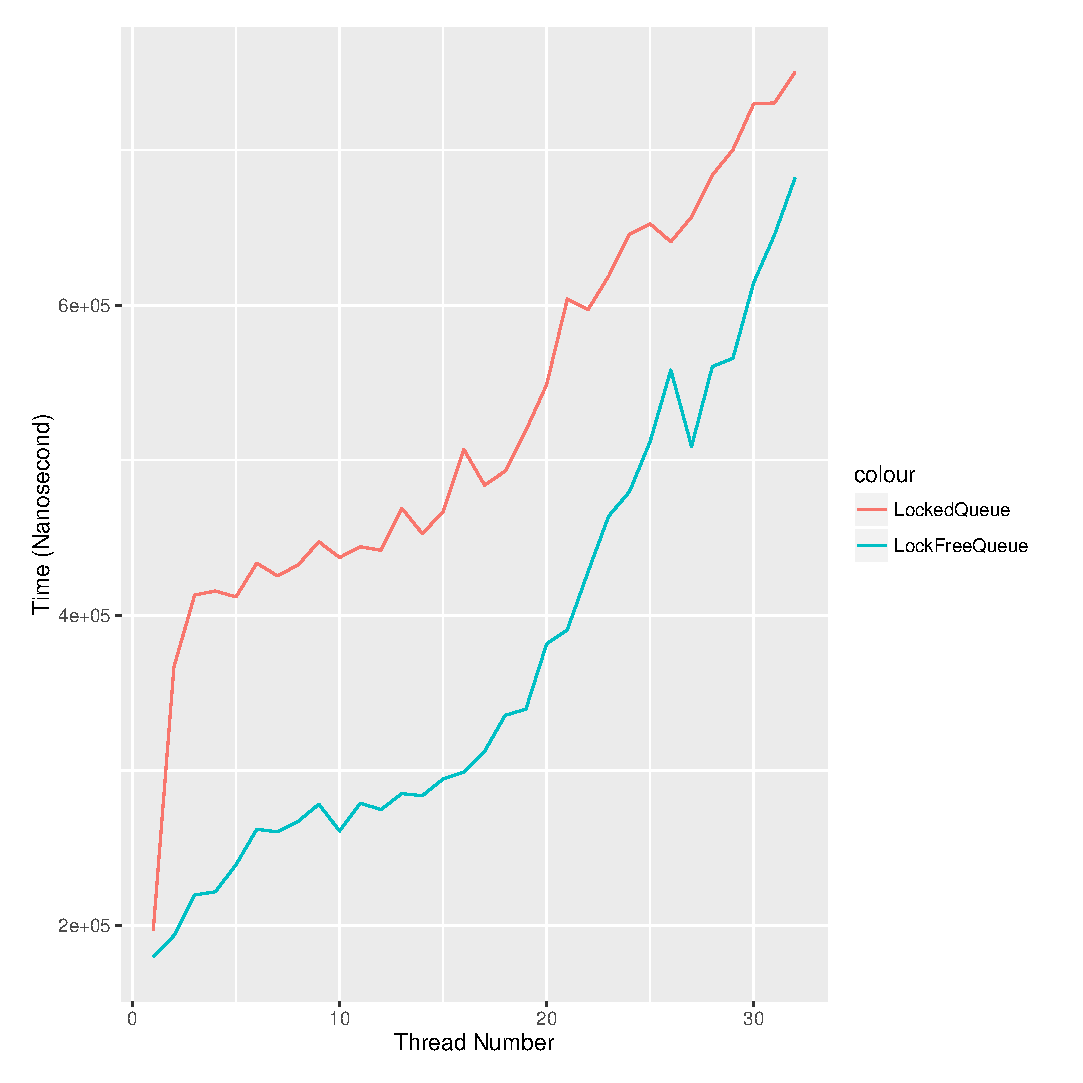
\includegraphics[scale=0.8]{result/result-tacc-7858356-mixed}
  \caption{Mixed Throughput}
\end{figure}

\section*{Results Analysis}
We can see that the result of both throughput nearly the same because in both implementation \lstinline{IsEmpty()} function are lock-free. So lock-free version's implementation does not enlarge the advantages in speed over the locked version in the mixed throughput. But these two throughput indeed distinct the performance of two implementations. We can clearly see that lock-free version has better performance than locked version over all thread number. It is what we expected.

\end{document}
